% !TEX root = ../thesis.tex
%
\tikzsetnextfilename{const-dos-approx-1}
%
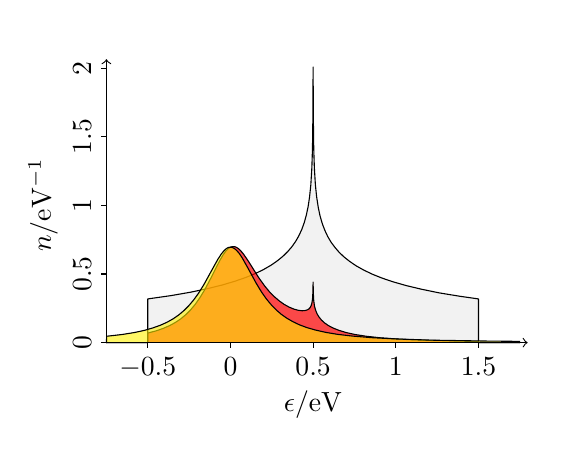
\begin{tikzpicture}[mark size=0.05cm, line cap=round]
	\draw [use as bounding box, draw=none]
		(-1.000, -1.000) rectangle +(6.750, 5.000);
	\draw [line join=round, fill opacity=0.05, fill=black] plot coordinates {
		(0.000, 0.000) (0.525, 0.000) (0.525, 0.555) (0.819, 0.597)
		(1.071, 0.641) (1.289, 0.687) (1.475, 0.733) (1.635, 0.781)
		(1.774, 0.829) (1.895, 0.879) (2.000, 0.931) (2.092, 0.984)
		(2.171, 1.039) (2.242, 1.097) (2.302, 1.156) (2.355, 1.217)
		(2.402, 1.284) (2.444, 1.357) (2.481, 1.437) (2.512, 1.523)
		(2.538, 1.616) (2.562, 1.729) (2.580, 1.850) (2.596, 2.004)
		(2.609, 2.218) (2.617, 2.463) (2.622, 2.851) (2.625, 3.500)
		(2.628, 2.851) (2.633, 2.463) (2.641, 2.218) (2.654, 2.004)
		(2.670, 1.850) (2.691, 1.714) (2.714, 1.606) (2.743, 1.507)
		(2.775, 1.424) (2.811, 1.347) (2.853, 1.276) (2.901, 1.211)
		(2.956, 1.147) (3.019, 1.087) (3.090, 1.031) (3.171, 0.976)
		(3.265, 0.923) (3.373, 0.871) (3.497, 0.821) (3.641, 0.772)
		(3.806, 0.725) (3.998, 0.679) (4.221, 0.633) (4.481, 0.590)
		(4.725, 0.555) (4.725, 0.000) (5.250, 0.000) };
	\draw [line join=round, fill opacity=0.7, fill=red] plot coordinates {
		(0.000, 0.000) (0.525, 0.000) (0.525, 0.122) (0.633, 0.150)
		(0.724, 0.182) (0.806, 0.218) (0.879, 0.258) (0.945, 0.303)
		(1.008, 0.355) (1.068, 0.415) (1.126, 0.484) (1.184, 0.566)
		(1.247, 0.669) (1.323, 0.813) (1.436, 1.036) (1.483, 1.117)
		(1.520, 1.167) (1.549, 1.195) (1.575, 1.212) (1.599, 1.220)
		(1.622, 1.220) (1.646, 1.213) (1.672, 1.197) (1.704, 1.169)
		(1.743, 1.122) (1.801, 1.037) (1.935, 0.824) (2.006, 0.725)
		(2.069, 0.648) (2.132, 0.584) (2.195, 0.530) (2.257, 0.486)
		(2.321, 0.451) (2.381, 0.426) (2.436, 0.411) (2.483, 0.405)
		(2.520, 0.407) (2.549, 0.415) (2.570, 0.427) (2.586, 0.444)
		(2.599, 0.467) (2.609, 0.500) (2.617, 0.548) (2.622, 0.629)
		(2.625, 0.768) (2.628, 0.623) (2.633, 0.534) (2.643, 0.461)
		(2.657, 0.412) (2.675, 0.367) (2.699, 0.327) (2.730, 0.288)
		(2.769, 0.252) (2.819, 0.217) (2.880, 0.185) (2.953, 0.156)
		(3.045, 0.128) (3.158, 0.103) (3.300, 0.081) (3.483, 0.061)
		(3.728, 0.044) (4.066, 0.029) (4.573, 0.018) (4.725, 0.015)
		(4.725, 0.000) (5.250, 0.000) };
	\draw [line join=round, fill opacity=0.6, fill=yellow] plot coordinates {
		(0.000, 0.000) (0.003, 0.081) (0.197, 0.103) (0.354, 0.128)
		(0.483, 0.156) (0.593, 0.188) (0.688, 0.222) (0.772, 0.260)
		(0.848, 0.303) (0.919, 0.352) (0.984, 0.407) (1.047, 0.470)
		(1.108, 0.542) (1.171, 0.629) (1.239, 0.739) (1.336, 0.916)
		(1.415, 1.058) (1.460, 1.127) (1.494, 1.168) (1.522, 1.194)
		(1.549, 1.208) (1.572, 1.212) (1.596, 1.209) (1.620, 1.199)
		(1.649, 1.176) (1.683, 1.138) (1.725, 1.076) (1.790, 0.960)
		(1.903, 0.753) (1.971, 0.641) (2.034, 0.552) (2.095, 0.479)
		(2.158, 0.414) (2.223, 0.358) (2.292, 0.310) (2.368, 0.266)
		(2.452, 0.226) (2.546, 0.191) (2.654, 0.160) (2.783, 0.131)
		(2.937, 0.105) (3.129, 0.083) (3.373, 0.063) (3.696, 0.046)
		(4.150, 0.031) (4.835, 0.020) (5.247, 0.016) (5.250, 0.000) };
	\draw [line cap=butt]
		(0.525, 0) -- +(0, -0.070) node [below] {$-0.5$}
		(1.575, 0) -- +(0, -0.070) node [below] {$0$}
		(2.625, 0) -- +(0, -0.070) node [below] {$0.5$}
		(3.675, 0) -- +(0, -0.070) node [below] {$1$}
		(4.725, 0) -- +(0, -0.070) node [below] {$1.5$}
		(0, 0.000) -- +(-0.070, 0) node [rotate=90, above] {$0$}
		(0, 0.872) -- +(-0.070, 0) node [rotate=90, above] {$0.5$}
		(0, 1.743) -- +(-0.070, 0) node [rotate=90, above] {$1$}
		(0, 2.615) -- +(-0.070, 0) node [rotate=90, above] {$1.5$}
		(0, 3.486) -- +(-0.070, 0) node [rotate=90, above] {$2$};
	\draw [<->, line cap=butt]
		(5.350, 0) -- (0, 0) -- (0, 3.600);
	\node [below=\baselineskip] at (2.625, -0.070)
		{$\epsilon / \mathrm{eV}$};
	\node [rotate=90, above=\baselineskip] at (-0.070, 1.750)
		{$n / \mathrm{eV^{-1}}$};
\end{tikzpicture}%
